\chapter{Deep Q-learning for RAM}\label{dqn-ram}
In our work, we adapt DQN to learn not from the game screens, but rather from the RAM~state of the Atari machine. In the following sections we describe the previous work in the domain of playing Atari games using RAM and the details of our approach.

\section{Related work}
In comparison to screen-based models, the models for playing Atari games based on RAM are not often studied in AI literature.

The work~\cite{nir} presents a classical planing algorithm to play Atari games based on the RAM. Since the RAM contains only $128$~bytes, one can efficiently search in this space. Nevertheless, the search is too slow to play in real-time---the evaluation of the method assume that one can spend as much time as it is needed to decide on a move. To the best of our knowledge, the only RAM-based agent that does not depend on search was presented in~\cite{ale}; we cite these results as~\texttt{ale\_ram}.

As the main benchmark of our work, we use original (screen-based) DQN model, introduced in~\cite{nips-dqn} and described in detail in chapter~\ref{dqn}. While it was improved in a number of ways in~\cite{nature-dqn, double-dqn, shallow-dqn, duelling-dqn}, leading to better architecture, hyperparameters, and Q-function estimates, these enhancements came at the cost of longer training time. Choosing a less sophisticated baseline~\cite{nips-dqn} makes it possible to fit a training of a single model in roughly $48$~hours using our technical setup (described in section~\ref{technical}) while still making it possible to verify feasibility of learning from RAM. We refer to this baseline architecture as~\texttt{nips}.

\section{Games}
We test our models on three games:
\begin{itemize}[itemindent=28pt]
  \item[\textbf{Bowling:}]{simulation of the game of bowling; the player aims the ball toward the pins and then steers the ball; the aim is to hit the pins~\cite{bowling,bowling_man}.}
  \item[\textbf{Breakout:}]{the player bounces the ball with the paddle towards the layer of bricks; the task is to destroy all bricks; a brick is destroyed when the ball hits it~\cite{breakout,breakout_man}.}
  \item[\textbf{Seaquest:}]{the player commands a submarine, which can shoot enemies and rescue divers by bringing them above the water-level; the player dies if he fails to get a diver up before the air level of submarine vanishes~\cite{seaquest,seaquest_man}.}
\end{itemize}
\begin{figure}
\begin{center}
\begin{subfigure}
  \centering
  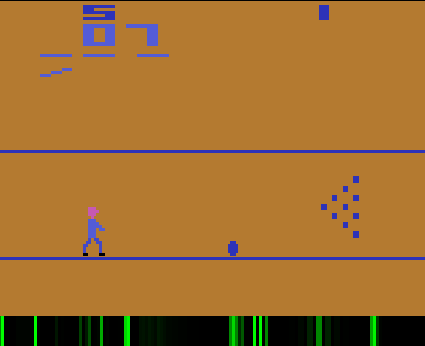
\includegraphics[width=.325\linewidth]{images/bowling1.png}
  \label{fig:sub1}
\end{subfigure}
\begin{subfigure}
  \centering
   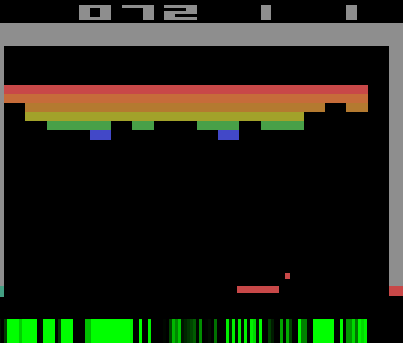
\includegraphics[width=.31\linewidth]{images/breakout2.png}
  \label{fig:sub2}
\end{subfigure}%
\begin{subfigure}
  \centering
  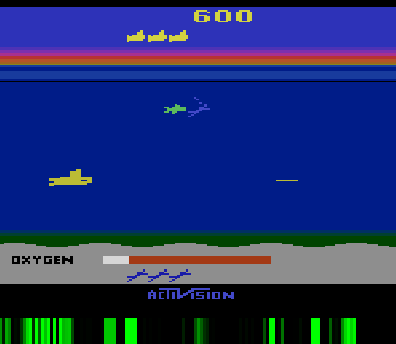
\includegraphics[width=.30\linewidth]{images/seaquest2.png}
  \label{fig:sub3}
\end{subfigure}
\caption{From left to right Bowling, Breakout and Seaquest. The $128$~vertical bars and the bottom of every screenshot represent the state of the memory, with black representing $0$ and lighter color corresponding to higher values of a given memory cell. }
\end{center}
\label{fig:screenshots}
\end{figure}

Each of this games offers a distinct challenge. Breakout is a relatively easy game with player's actions limited to moves along the horizontal axis. We picked Breakout because disastrous results of learning would indicate a fundamental problem with the RAM learning.

The deep Q-network for Seaquest constructed in~\cite{nips-dqn} plays at an amateur human level and for this reason we consider this game as a tempting target for improvements. The game state has also some elements that possibly can be detected by the RAM-only network (e.g. oxygen-level meter or the number of picked divers).

Bowling seems to be a hard game for all deep Q-network models. It is an interesting target for the RAM-based networks, because visualizations suggest that only a couple of RAM~cells are changing during play.

\section{Technical infrastructure}\label{technical}
For our experiments we adapted Nathan~Sprague's implementation of deep Q-learning~\cite{sprague} in Theano~\cite{theano} and Lasagne~\cite{lasagne}. The code used for experiment uses Arcade~Learning~Environment~\cite{ale} for communicating with an Atari simulator, but we also integrated our code with OpenAI~gym, which is a wrapper on top of~ALE. Our code can be found on github~\cite{our-dqn} (as well as in the directory \texttt{code/dqn} on the CD).

The experiments were performed on a GPU cluster of Interdisciplinary Centre for Mathematical and Computational Modelling using Linux machines equipped with NVIDIA~GTX~$480$. Each of them lasted $1$--$3$~days, with the screen-only models taking approximately twice as much time to train as RAM-only ones. The details of using the cluster's architecture can be found in appendix~\ref{icm}.

\section{Hyperparameters and network architectures}
\SetAlgorithmName{Neural network}{List of Neural networks}

We have evaluated the performance of the DQN method for two neural network architectures. They serve as a Q-value approximator: accepting RAM as the input and returning estimates of Q-values of each possible action. We also made a limited number of experiments using networks accepting as an input both RAM and screen, which are described in section~\ref{screen-ram-networks}.

All the hyperparameters of the models we consider are the same as in~\cite{nips-dqn} if not mentioned otherwise (see appendix~\ref{hyperparams}). One change we made is to decrease of the size of the replay memory (see section~\ref{experience-replay}) to $10^5$~observations, so that it fits $1.5$GB of~NVIDIA~GTX~$480$ memory.\footnote{We made experiments with replay memory size of~$5\cdot 10^5$ and have not observed a statistically significant change in results.}

We also decided to pass to the network only the RAM state corresponding to the last timestep before agent's action (and not $4$, as in~\cite{nips-dqn}, compare section~\ref{dqn-frameskip}), as the reason to pass multiple frames as an input---violation of markovian property of environment---is void with RAM inputs.
Basic experiments we performed suggest it was a good decision, as passing the last couple of RAM frames obstructed the learning procedure and worsened the results.
We still used non-unity frameskip though: it is further discussed in section~\ref{our-frameskip}.

The RAM input to the network was scaled by~$256$, to make all the inputs lie between $0$ and $1$.

\subsection{\texttt{just\_ram}}
The first proposed architecture is a small $2$~hidden layer network with rectified linear units as an activation function.
%%%%%%%%%%%%%%%%%%%%%%%%%%%%%%%%%%%%%%%%%%%%%%%%%%%%%%%%%

\RestyleAlgo{ruled}
\begin{algorithm}[H]
\SetAlgoRefName{1}
\DontPrintSemicolon
\AlFnt{\small\sf}
\caption{\texttt{just\_ram} (numActions)}
% \LinesNumbered
\SetAlgoVlined

\AlFnt{\small\sf}
\KwIn{RAM} 
\KwOut{A vector of length numActions}
\vspace{0.05cm}
hiddenLayer1 $\leftarrow$ DenseLayer(RAM, $128$, rectify)\;
hiddenLayer2 $\leftarrow$ DenseLayer(hiddenLayer1, $128$, rectify)\;
output $\leftarrow$ DenseLayer(hiddenLayer2, numActions, no activation)\;

\Return{{\upshape output}}
\end{algorithm}
%%%%%%%%%%%%%%%%%%%%%%%%%%%%%%%%%%%%%%%%%%%%%%%%%%%%%%%%%
\subsection{\texttt{big\_ram}}
The second architecture consists of $4$ hidden layers.


%%%%%%%%%%%%%%%%%%%%%%%%%%%%%%%%%%%%%%%%%%%%%%%%%%%%%%%%%
\begin{algorithm}[H]
\SetAlgoRefName{2}  % TODO: introduce a proper latex counter
\DontPrintSemicolon
\AlFnt{\small\sf}
\caption{\texttt{big\_ram} (numActions)}

\SetAlgoVlined
% \LinesNumbered

\KwIn{RAM} 
\KwOut{A vector of length numActions}
\vspace{0.05cm}

hiddenLayer1 $\leftarrow$ DenseLayer(RAM, $128$, rectify)\;
hiddenLayer2 $\leftarrow$ DenseLayer(hiddenLayer1, $128$, rectify)\;
hiddenLayer3 $\leftarrow$ DenseLayer(hiddenLayer2, $128$, rectify)\;
hiddenLayer4 $\leftarrow$ DenseLayer(hiddenLayer3, $128$, rectify)\;
output $\leftarrow$ DenseLayer(hiddenLayer4, numActions, no activation)\;

\Return{{\upshape output}}
\end{algorithm}

\section{Evaluation method}
The process of evaluating the RAM version of DQN is divided in experiments. By one experiment we mean a full training of a single deep Q-network in a fixed game. The training consists of $100$~epochs, each containing a training and testing part.

During a training part of an epoch, agent plays the game for a couple of episodes (full games) for a total of $50000$~steps, choosing actions based on his Q-function estimate in each step (using $\varepsilon$-greedy strategy). After a step, the learning algorithm performs one step of parameter optimization, using gradients of the loss function of the random $32$~observations\footnote{This hyperparameter is mentioned as \texttt{BATCH\_SIZE} in the code and the hyperparameter table.} (observations contain the RAM~state before the action, the action itself, the reward achieved and the RAM state after the action) from the replay memory.

After a training part, we perform a testing part of an epoch. It consists of playing a trained agent for $10000$~steps using $\varepsilon=0.05$ without changing its parameters, only to evaluate its current performance. This number of steps usually covered around $10$--$20$ game episodes.

The numerical result of an experiment we present thorough this work is the average cumulative (non-discounted) reward in episode during a best testing epoch. To make sure this is a reliable metric, we performed experiments in Breakout involving testing the network with best-epoch parameters on a couple different random seeds (a given game episode is initialized randomly, to make games slightly different each time they are played) for $100000$~steps. The results of this evaluation were consistently lower by about~$30\%$ among all of the methods we tried, including~\texttt{nips}.

\section{Results of the basic method}
The evaluation results during the course of training in all three games of the basic methods described above (\texttt{nips}, \texttt{just\_ram}, \texttt{big\_ram}) are presented in figures \labelcref{fig:breakout-plain,fig:seaquest-plain,fig:bowling-plain}.

\begin{figure}[h]
\centering
\begin{tikzpicture}[scale=1]
\begin{axis}[
   xlabel={Training epoch},
   ylabel={Average score per episode},
   xmin=0,xmax=101,
   x=0.12cm,
   grid=major,
   mark options={solid, scale=0.35},
   legend entries={\texttt{nips}, \texttt{just\_ram}, \texttt{big\_ram}},
   legend style={legend pos=north west},
]
\addplot[mark=*, color=black, line width=0.25pt] table {experiments/breakout_nips.txt};
\addplot[mark=*, color=blue, line width=0.25pt] table {experiments/breakout_just_ram_100.txt};
h\addplot[mark=*, color=red, line width=0.25pt] table {experiments/breakout_big_ram_100.txt};
\addplot[mark=*, color=black, only marks, mark size=5] table {
x y
86 213.1428571
};
\addplot[mark=*, color=blue, only marks, mark size=5] table {
x	y
84	99.55555556
};
\addplot[mark=*, color=red, only marks, mark size=5] table {
x	y
50	178
};
\end{axis}
\end{tikzpicture}
\caption{Training results for Breakout for three basic models: \texttt{nips}, \texttt{just\_ram}, \texttt{big\_ram}. }
\label{fig:breakout-plain}
\end{figure}

\begin{figure}[h]
\centering
\begin{tikzpicture}[scale=1]
\begin{axis}[
   xlabel={Training epoch},
   ylabel={Average score per episode},
   xmin=0,xmax=101,
   x=0.12cm,
   grid=major,
   mark options={solid, scale=0.35},
   legend entries={\texttt{nips}, \texttt{just\_ram}, \texttt{big\_ram}},
   legend style={legend pos=north west},
]
\addplot[mark=*, color=black, line width=0.25pt] table {experiments/seaquest_nips.txt};
\addplot[mark=*, color=blue, line width=0.25pt] table {experiments/seaquest_just_ram_100.txt};
\addplot[mark=*, color=red, line width=0.25pt] table {experiments/seaquest_big_ram_100.txt};
\addplot[mark=*,color=black, only marks,mark size=5] table {
x y
82 1808
};
\addplot[mark=*, color=blue, only marks, mark size=5] table {
x y
90	1360
};
\addplot[mark=*, color=red, only marks, mark size=5] table {
x y
88	2680
};
\end{axis}
\end{tikzpicture}
\caption{Training results for Seaquest three basic models: \texttt{nips}, \texttt{just\_ram}, \texttt{big\_ram}.}
\label{fig:seaquest-plain}
\end{figure}

\begin{figure}[h]
\centering
\begin{tikzpicture}[scale=1]
\begin{axis}[
   xlabel={Training epoch},
   ylabel={Average score per episode},
   xmin=0,xmax=101,
   x=0.12cm,
   grid=major,
   mark options={solid, scale=0.35},
   legend entries={\texttt{nips}, \texttt{just\_ram}, \texttt{big\_ram}},
   legend style={legend pos=north west},
]
\addplot[mark=*, color=black, line width=0.25pt] table {experiments/bowling_nips.txt};
\addplot[mark=*, color=blue, line width=0.25pt] table {experiments/bowling_just_ram_100.txt};
\addplot[mark=*, color=red, line width=0.25pt] table {experiments/bowling_big_ram_100.txt};
\addplot[mark=*, color=black, only marks, mark size=5] table {
x y
71	54
};
\addplot[mark=*, color=blue, only marks, mark size=5] table {
x	y
66	58.25
};
\addplot[mark=*, color=red, only marks, mark size=5] table {
x	y
59 66.25
};
\end{axis}
\end{tikzpicture}
\caption{Training results for Bowling  for three basic models: \texttt{nips}, \texttt{just\_ram}, \texttt{big\_ram}.}
\label{fig:bowling-plain}
\end{figure}

The best epoch results of these methods, along with \texttt{ale\_ram}\footnote{The \texttt{ale\_ram}'s evaluation method differ---the scores presented are the average over $30$ trials consisting of a long period of learning and then a long period of testing, nevertheless the results are much worse than of any DQN-based method presented here.} are summarized in table~\ref{table:results-plain}.
\begin{table}[h]
\centering
  \begin{tabular}{X c c c c}
  \toprule
  & Breakout & Seaquest & Bowling  \\
  \midrule
  \texttt{nips} best & \textbf{213.14}  & $1808$  & $54.0$  \\
  \texttt{just\_ram} best & $99.56$ & $1360$ & $58.25$  \\
  \texttt{big\_ram} best & $178.0$ & \textbf{2680} & \textbf{66.25} \\
  \texttt{ale\_ram} & $4.0$ & $593.7$ & $29.3$ \\
  \bottomrule
  \end{tabular}
\caption{Table summarizing test results for basic methods.}
\label{table:results-plain}
\end{table}

In Breakout, the best results for the \texttt{big\_ram}~model is weaker than one obtained by screen-only network \texttt{nips}. In Seaquest the \texttt{big\_ram}~model was better, and \texttt{just\_ram} worse than \texttt{nips}, while in Bowling both RAM-based models performed better than screen-based \texttt{nips}.
The training plots show that there is a big variance of the results between training epochs.
